\documentclass[10pt]{standalone}

\usepackage[english]{babel}
\usepackage{amsmath,amsthm,amssymb,amsfonts}
\usepackage[italicdiff]{physics}
\usepackage[T1]{fontenc}
\usepackage{lmodern}
\usepackage[dvipsnames]{xcolor}
\usepackage[utf8]{inputenc}
\usepackage{tikz,tikz-3dplot,tikz-cd,pgf,pgfplots}
\usetikzlibrary{arrows.meta}
\pgfplotsset{compat=newest}

\setlength{\parindent}{0pt}

% Created by Senan Sekhon, August 7, 2021

\begin{document}

\thispagestyle{empty}

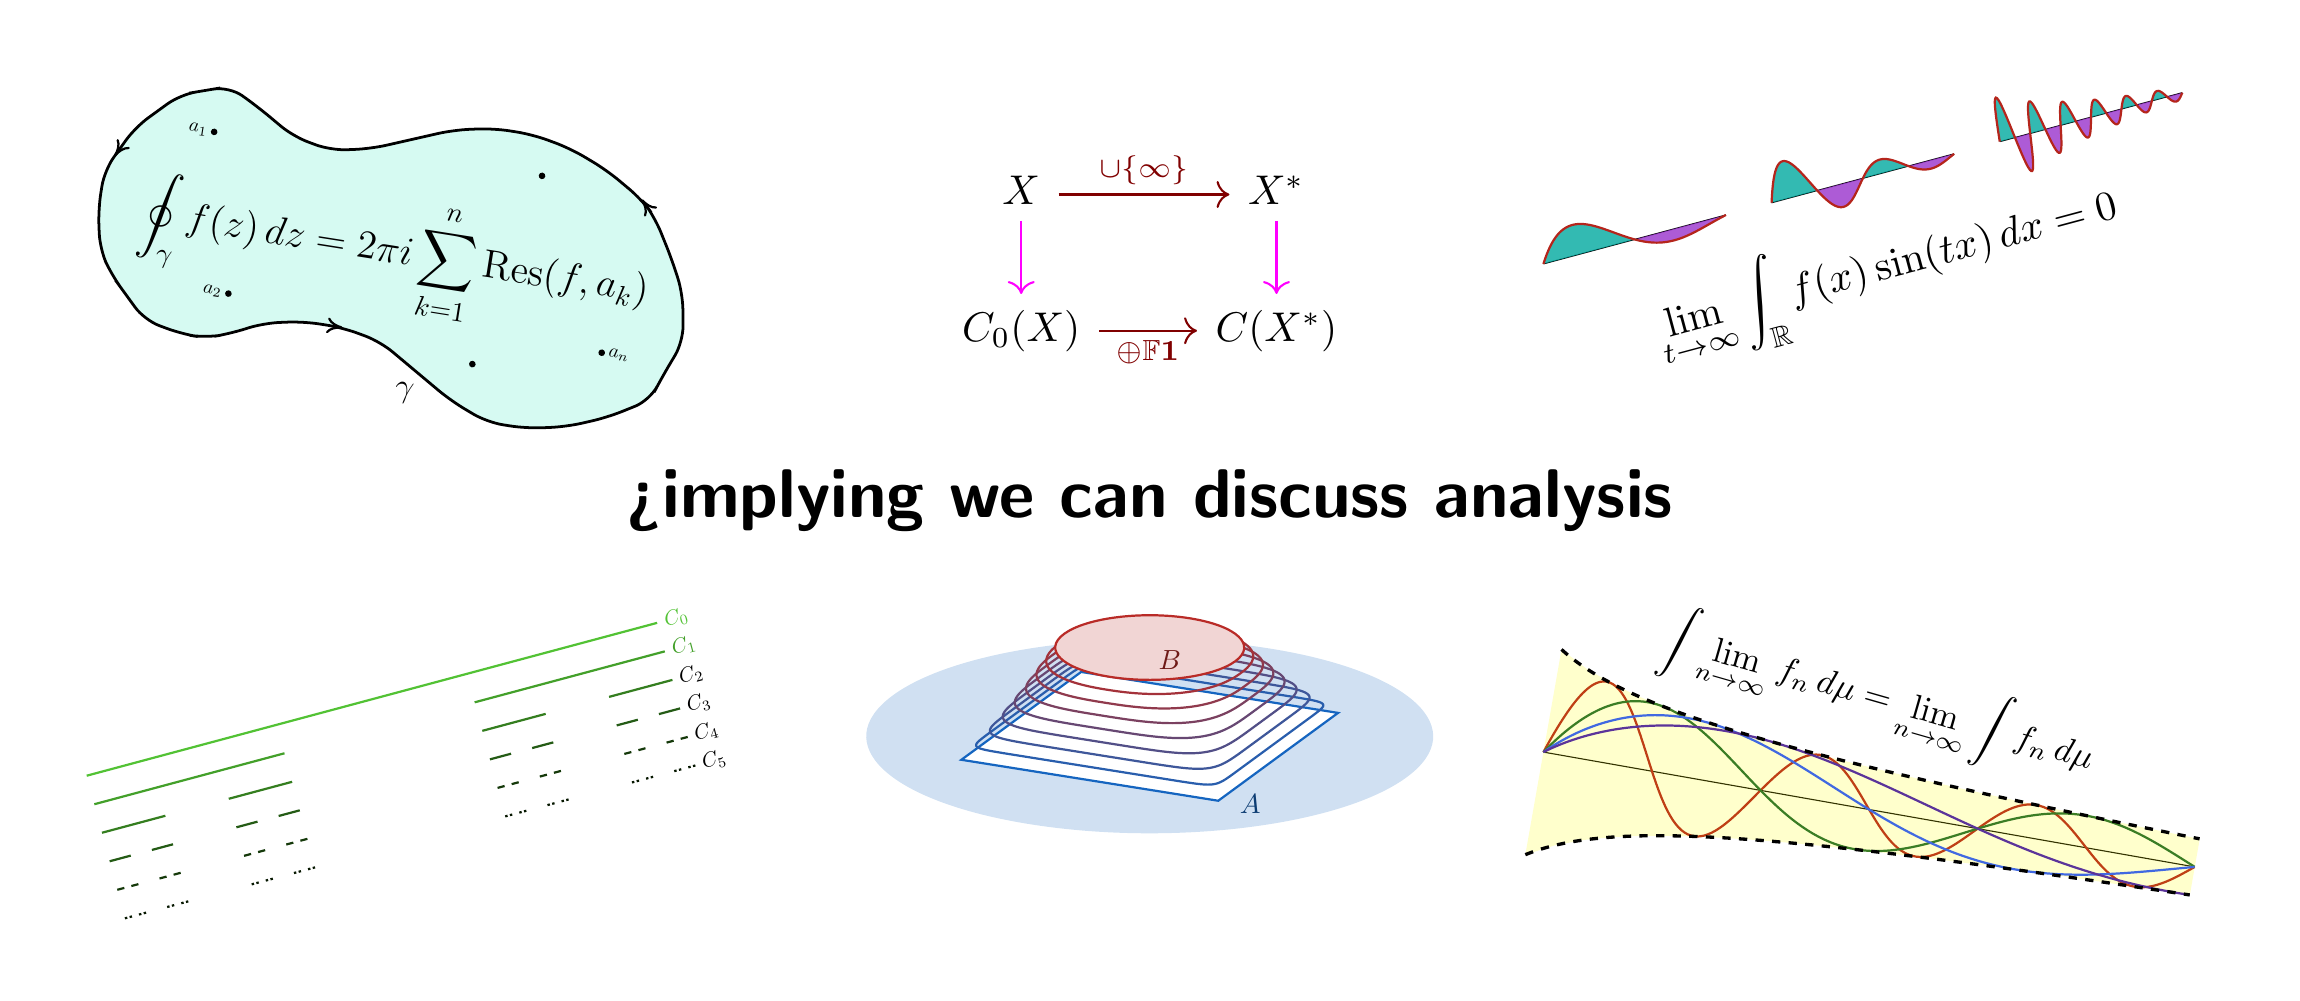
\begin{tikzpicture}[urysohn_lemma/.pic={%%% Urysohn's Lemma (this cannot be drawn in the main body as it is a tikz3d picture)
    \tdplotsetmaincoords{70}{115}
    \begin{scope}[tdplot_main_coords]
        \definecolor{acol}{HTML}{1565C0} %color for region A
        \definecolor{bcol}{HTML}{B92B27} %color for region B
        \begin{scope}[canvas is xy plane at z=0]
            \fill[acol!20,even odd rule] (0,0) circle (3) (-1.5,-1.5) rectangle (1.5,1.5);
            \draw[thick,acol] (-1.5,-1.5) rectangle (1.5,1.5);
        \end{scope}
    \pgfmathtruncatemacro{\n}{8}
    \foreach \i in {1,...,\number\numexpr\n-1\relax}
    {
        \pgfmathsetmacro{\h}{\i/\n} % Height above xy plane (z-value)
        \begin{scope}[canvas is xy plane at z=\h]
            \pgfmathsetmacro{\d}{100*\h} % Partial opacity of acol
            \draw[thick,smooth,bcol!\d!acol,domain=0:3*pi,samples=200] plot ({(3-\h)/2*cos(deg(\x))*abs(cos(deg(\x)))^(\h-1)},{(3-\h)/2*sin(deg(\x))*abs(sin(deg(\x)))^(\h-1)}); % Domain set to [0,3*pi] to avoid gaps at the endpoints
        \end{scope}
    }
    \begin{scope}[canvas is xy plane at z=1]
        \draw[thick,bcol,fill=bcol!20] (0,0) circle (1);
    \end{scope}
    \node[acol!60!black] at (1.45,1.85,0) {$A$};
    \node[bcol!60!black] at (0.25,0.35,1) {$B$};
    \end{scope}
}]

    %%% Border for cover photo (to be cropped out)
    \clip (-14.25,-6) rectangle (14.25,6); % Approximate proportions for a Facebook cover photo

    %%% Diagram for Residue Theorem
    \begin{scope}[shift={(-9.6,3.1)},rotate=-9,scale=1,every node/.style={transform shape}]
        % \definecolor{ext}{HTML}{FF8235} % Color for exterior of gamma
        \definecolor{int}{HTML}{30E8BF} % Color for interior of gamma
        % \draw[step=0.5,gray,thin] (-4.5,-2.5) grid (4.5,2.5); % Fine grid for drawing aid
        % \draw[step=1,gray,thick] (-4,-2) grid (4,2); % Coarse grid for drawing aid
        % \fill[ext!40] (-4.5,-2.5) rectangle (4.5,2.5);
        \draw[-,line width=1pt,rounded corners=2mm,fill=int!20] (0,-1.1) -- (0.5,-1.4) -- (1,-1.7) -- (1.5,-1.9) -- (2,-1.9) -- (2.5,-1.8) -- (3,-1.6) -- (3.5,-1.3) -- (3.6,-1) -- (3.8,-0.5) -- (3.7,0.1) -- (3.5,0.5) -- (3.2,1) -- (3,1.2) -- (2.5,1.5) -- (2,1.7) -- (1.5,1.8) -- (1,1.8) -- (0.5,1.7) -- (0,1.5) -- (-0.5,1.3) -- (-1,1.2) -- (-1.5,1.3) -- (-2,1.6) -- (-2.4,1.8) -- (-2.7,1.7) -- (-3,1.6) -- (-3.5,1.1) -- (-3.8,0.5) -- (-3.8,0) -- (-3.7,-0.5) -- (-3.5,-0.8) -- (-3.3,-1) -- (-3,-1.3) -- (-2.5,-1.4) -- (-2.2,-1.4) -- (-1.9,-1.3) -- (-1.5,-1.1) -- (-1,-1) -- (-0.5,-1) -- cycle;
        \fill (-2.5,1.2) circle (1.2pt) node[left,scale=0.7]{$a_1$};
        \fill (-2,-0.8) circle (1.2pt) node[left,scale=0.7]{$a_2$};
        \fill (1.2,-1.2) circle (1.2pt);
        \fill (2.8,-0.8) circle (1.2pt) node[right,scale=0.7]{$a_n$};
        \fill (1.7,1.3) circle (1.2pt);
        \node[font=\large] at (0.4,-1.7) {$\gamma$};
        \draw[arrows={->[line width=0.8pt,length=2mm,width=2mm]}] (3.1,1.1) -- (3,1.2);
        \draw[arrows={->[line width=0.8pt,length=2mm,width=2mm]}] (-3.6,0.9) -- (-3.7,0.7);
        \draw[arrows={->[line width=0.8pt,length=2mm,width=2mm]}] (-0.6,-1) -- (-0.5,-1);
        \node[font=\Large] at (0,0) {$\displaystyle\oint_\gamma f(z)\,dz=2\pi i\sum_{k=1}^n \operatorname{Res}(f,a_k)$};
    \end{scope}

    %%% Diagram for Unitization of C_0(X)
    \node at (0,3) {
        \begin{tikzcd}[transform canvas={scale=1.5},arrows={line width=0.5pt}]
            X \arrow[r,Maroon,"\cup\{\infty\}"] \arrow[d,Fuchsia] & X^* \arrow[d,Fuchsia] \\
            C_0(X) \arrow[r,Maroon,"\oplus\mathbb{F}\textbf{1}"'] & C(X^*)
        \end{tikzcd}
    };

    %%% Diagram for Riemann-Lebesgue Lemma
    \begin{scope}[shift={(5,3)},rotate=15,scale=1.5,every node/.style={transform shape}]
        \newcommand{\areas}[1][1]{ % Template for graph
            \pgfmathtruncatemacro{\n}{#1} % Number of periods of sine wave in graph
            \draw (0,0) -- (4,0);
            % \draw (0,-1) -- (0,1);
            \foreach \i in {1,...,\n}
            {
                \fill[smooth,Emerald,fill opacity=0.8,domain={(4*\i-4)/\n}:{(4*\i-2)/\n},variable=\x] ({(4*\i-4)/\n},0) -- plot ({\x},{exp(-\x/2)*sin(\n*90*\x)}) -- ({(4*\i-2)/\n},0) -- cycle;
                \fill[smooth,DarkOrchid,fill opacity=0.8,domain={(4*\i-2)/\n}:{4*\i/\n},variable=\x] ({(4*\i-2)/\n},0) -- plot ({\x},{exp(-\x/2)*sin(\n*90*\x)}) -- ({4*\i/\n},0) -- cycle;
            }
            \draw[thick,smooth,BrickRed,domain=0:4,samples=200] plot (\x,{exp(-\x/2)*sin(\n*90*\x)});
        }
        \begin{scope}[shift={(0,0)},scale=0.4]
            \areas[1]
        \end{scope}
        \begin{scope}[shift={(2,0)},scale=0.4]
            \areas[2]
        \end{scope}
        \begin{scope}[shift={(4,0)},scale=0.4]
            \areas[6]
        \end{scope}
        \node at (2.8,-0.8) {$\displaystyle\lim_{t\to\infty} \int_\mathbb{R} f(x)\sin(tx)\,dx=0$};
    \end{scope}

    %%% Diagram for Cantor Set
    \begin{scope}[shift={(-13.5,-3.5)},rotate=15,scale=7.5,every node/.style={transform shape,scale=0.1}] %Scale for nodes set to 0.1 to adjust relative size
        \definecolor{col1}{HTML}{52C234} %color for C_0
        \definecolor{col2}{HTML}{061700} %color for C_5
        % C_0
        \draw[thick,col1] (0,0) -- (1,0) node[right]{$C_0$};
        % C_1
        \draw[thick,col1!80!col2] (0,-1/20) -- (1/3,-1/20);
        \draw[thick,col1!80!col2] (2/3,-1/20) -- (1,-1/20) node[right]{$C_1$};
        % C_2
        \foreach \x in {0,2}
        \draw[thick,col1!60!col2] ({\x/3},-1/10) -- ({(3*\x+1)/9},-1/10);
        \foreach \x in {0,2}
        \draw[thick,col1!60!col2] ({(3*\x+2)/9},-1/10) -- ({(\x+1)/3},-1/10);
        \node[right] at (1,-1/10) {$C_2$};
        % C_3
        \foreach \x in {0,2,6,8}
        \draw[thick,col1!40!col2] ({\x/9},-3/20) -- ({(3*\x+1)/27},-3/20);
        \foreach \x in {0,2,6,8}
        \draw[thick,col1!40!col2] ({(3*\x+2)/27},-3/20) -- ({(\x+1)/9},-3/20);
        \node[right] at (1,-3/20) {$C_3$};
        % C_4
        \foreach \x in {0,2,6,8,18,20,24,26}
        \draw[thick,col1!20!col2] ({\x/27},-1/5) -- ({(3*\x+1)/81},-1/5);
        \foreach \x in {0,2,6,8,18,20,24,26}
        \draw[thick,col1!20!col2] ({(3*\x+2)/81},-1/5) -- ({(\x+1)/27},-1/5);
        \node[right] at (1,-1/5) {$C_4$};
        % C_5
        \foreach \x in {0,2,6,8,18,20,24,26,54,56,60,62,72,74,78,80}
        \draw[thick,col2] ({\x/81},-1/4) -- ({(3*\x+1)/243},-1/4);
        \foreach \x in {0,2,6,8,18,20,24,26,54,56,60,62,72,74,78,80}
        \draw[thick,col2] ({(3*\x+2)/243},-1/4) -- ({(\x+1)/81},-1/4);
        \node[right] at (1,-1/4) {$C_5$};
    \end{scope}

    %%% Diagram for Urysohn's Lemma
    \draw (0,-3) pic[scale=1.2]{urysohn_lemma};

    %%% Diagram for Dominated Convergence Theorem
    \begin{scope}[shift={(5,-3.2)},rotate=-10,scale=0.7,every node/.style={transform shape}]
        \draw[-] (0,0) -- (12,0);
        \pgfmathdeclarefunction{dom}{1}{\pgfmathparse{3*(#1+2)^(-2/3)}};
        \fill[Yellow,fill opacity=0.2,domain=0:12,variable=\x] (0,0) -- plot ({\x},{dom(\x)}) -- (12,0) -- plot ({12-\x},{-dom(12-\x)}) -- cycle;
        \draw[thick,Bittersweet,smooth,domain=0:12,samples=200] plot (\x,{dom(\x)*sin(90*\x)});
        \draw[thick,OliveGreen,smooth,domain=0:12,samples=200] plot (\x,{dom(\x)*sin(45*\x)});
        \draw[thick,RoyalBlue,smooth,domain=0:12,samples=200] plot (\x,{dom(\x)*sin(30*\x)});
        \draw[thick,RoyalPurple,smooth,domain=0:12,samples=200] plot (\x,{dom(\x)*sin(45/2*\x)});
        \draw[very thick,smooth,dashed,domain=0:12,samples=200] plot (\x,{dom(\x)});
        \draw[very thick,smooth,dashed,domain=0:12,samples=200] plot (\x,{-dom(\x)});
        \node[rotate=-6,scale=1.8] at (5.8,2) {$\displaystyle\int\lim_{n\to\infty} f_n\,d\mu=\lim_{n\to\infty} \int f_n\,d\mu$};
    \end{scope}

    %%% Title
    \node[font=\fontsize{28}{28}\sffamily\bfseries] at (0,0) {>implying we can discuss analysis};
\end{tikzpicture}

\end{document}